\documentclass[12pt,english,french,twoside]{report}\usepackage[]{graphicx}\usepackage[]{color}
%% maxwidth is the original width if it is less than linewidth
%% otherwise use linewidth (to make sure the graphics do not exceed the margin)
\makeatletter
\def\maxwidth{ %
  \ifdim\Gin@nat@width>\linewidth
    \linewidth
  \else
    \Gin@nat@width
  \fi
}
\makeatother

\definecolor{fgcolor}{rgb}{0.345, 0.345, 0.345}
\newcommand{\hlnum}[1]{\textcolor[rgb]{0.686,0.059,0.569}{#1}}%
\newcommand{\hlstr}[1]{\textcolor[rgb]{0.192,0.494,0.8}{#1}}%
\newcommand{\hlcom}[1]{\textcolor[rgb]{0.678,0.584,0.686}{\textit{#1}}}%
\newcommand{\hlopt}[1]{\textcolor[rgb]{0,0,0}{#1}}%
\newcommand{\hlstd}[1]{\textcolor[rgb]{0.345,0.345,0.345}{#1}}%
\newcommand{\hlkwa}[1]{\textcolor[rgb]{0.161,0.373,0.58}{\textbf{#1}}}%
\newcommand{\hlkwb}[1]{\textcolor[rgb]{0.69,0.353,0.396}{#1}}%
\newcommand{\hlkwc}[1]{\textcolor[rgb]{0.333,0.667,0.333}{#1}}%
\newcommand{\hlkwd}[1]{\textcolor[rgb]{0.737,0.353,0.396}{\textbf{#1}}}%

\usepackage{framed}
\makeatletter
\newenvironment{kframe}{%
 \def\at@end@of@kframe{}%
 \ifinner\ifhmode%
  \def\at@end@of@kframe{\end{minipage}}%
  \begin{minipage}{\columnwidth}%
 \fi\fi%
 \def\FrameCommand##1{\hskip\@totalleftmargin \hskip-\fboxsep
 \colorbox{shadecolor}{##1}\hskip-\fboxsep
     % There is no \\@totalrightmargin, so:
     \hskip-\linewidth \hskip-\@totalleftmargin \hskip\columnwidth}%
 \MakeFramed {\advance\hsize-\width
   \@totalleftmargin\z@ \linewidth\hsize
   \@setminipage}}%
 {\par\unskip\endMakeFramed%
 \at@end@of@kframe}
\makeatother

\definecolor{shadecolor}{rgb}{.97, .97, .97}
\definecolor{messagecolor}{rgb}{0, 0, 0}
\definecolor{warningcolor}{rgb}{1, 0, 1}
\definecolor{errorcolor}{rgb}{1, 0, 0}
\newenvironment{knitrout}{}{} % an empty environment to be redefined in TeX

\usepackage{alltt}
\usepackage[francais]{babel}
\usepackage[T1]{fontenc}
\usepackage{lmodern}
\usepackage[utf8]{inputenc}
% inclu un fichier de bibliothèques
\include{rpu-2012.sty}

% la directive suivante permet d'utiliser le séparateur de milliers. 
%Deux formulation sont utilisables mais exclusives l'une de l'autre. L'instruction "autolanguage" permet d'utiliser \nombre{} ou \np{}
% exemple: L'ensemble des SU ont déclaré \np{length(e)} passages en 2013
%\usepackage{numprint}
\usepackage[autolanguage,np]{numprint}

% la ligne qui suit donne un titre interne au document pdf et crée des liens cliquables en bleu sur les tables et figures
\usepackage[pdftitle={RPU2012-Resural}, colorlinks=true, linkcolor=blue,citecolor=blue, urlcolor=blue, linktocpage=true, breaklinks=true]{hyperref}

\usepackage[left=4cm,right=3cm,top=2cm,bottom=2cm]{geometry}
\usepackage{graphicx}

\usepackage{amsmath}
\usepackage{amsfonts}
\usepackage{amssymb}
\usepackage{xcolor} 
\usepackage{hyperref} 
\usepackage{tikz} 
\usepackage{fancyvrb}

\usepackage{makeidx}
\makeindex

\bibliographystyle{plain}

\makeglossary
%\makeindex -s glossaire.ist RPU2013.glo -o RPU2013.glx

% \newenvironment{leglossaire}{\begin{list}{}{%
%   \setlength{\labelwidth}{.5\textwidth}%
%   \setlength{\labelsep}{-.8\labelwidth}%
%   \setlength{\itemindent}{\parindent}%
%   \setlength{\leftmargin}{25pt}%
%   \setlength{\rightmargin}{0pt}%
%   \setlength{\itemsep}{.8\baselineskip}%
%   \renewcommand{\makelabel}[1]{\boiteentreeglossaire{##1}}}}
% {\end{list}}
%       
% \newcommand{boiteentreeglossaire}[1]{%
%   \parbox[b]{\labelwidth}{%
%   \setlength{\fboxsep}{3pt}%
%   \setlength{\fboxrule}{.4pt}%
%   \shadow{\sffamily#1}\\\hfill\mbox{}}}

% Définitions de constantes


\IfFileExists{upquote.sty}{\usepackage{upquote}}{}


\begin{document}

\title{Analyse des données RPU 2013 de la région Alsace}
\author{RESURAL\thanks{Réseau des urgences en Alsace - Equipe de coordination Dr J.C.
Bartier \& Madame Christine Hecker}}
\date{\today}
\maketitle

%\SweaveOpts{concordance=TRUE}
%\SweaveOpts{fig.path='./figure/rpu2013-', comment=NA, prompt=FALSE}

\tableofcontents
\listoftables
\listoffigures



%======================================================== PARTIE 1
\part{Le Réseau des urgences en Alsace}
\chapter{Historique}
utilisation de la directive \\nombre{}, par exemple: 
Un grand nombre 300000 et avec séparation des milliers \nombre{300000}

La même chose avec \\np{}: 
Un grand nombre 300000 et avec séparation des milliers \np{300000}

\chapter{Organisation géographique}

% geographie.Rnw

L'Alsace est la plus petite région de France (n°42) avec la Corse. Elle est formée de deux départements, le bas-Rhin (67) et le haut-Rhin (68), sont les chef-lieu sont respectivement Strasbourg et Colmar.

\section{Les secteurs sanitaires}

L'alsace est divisée en quatre secteurs sanitaires
\begin{enumerate}
  \item secteur 1: Haguenau, Wissembourg et Saverne
  \item secteur 2: Strasbourg
  \item secteur 3: Sélestat et Colmar
  \item secteur 4: Mulhouse
\end{enumerate}

\section{Les zones de proximité}

Il existe neuf territoires de proximité:
\begin{enumerate}
  \item territoire 1: Wissembourg
  \item territoire 2: Haguenau
  \item territoire 3: Saverne
  \item territoire 4: Strasbourg
  \item territoire 5: Molsheim-Schirmeck
  \item territoire 6: Sélestat-Obernai
  \item territoire 7: Colmar
  \item territoire 8: Guebwiller
  \item territoire 9: Thann
  \item territoire 10: Mulhouse
  \item territoire 11: Altkirch
  \item territoire 12: Saint-Louis
\end{enumerate}

\section{Démographie}
\subsection{Généralités}
En France, les populations légales sont calculées par l'INSEE sur la base de définitions réglementaires à partir de recensement de la population. Ce document utilise la \emph{Population municipale} \ref{Population_municipale} \index{Population@Population!municipale}  qui est la nouvelle dénomination de la population sans double comptes. Le chiffre est donc inférieur de celui de la \emph{Population totale} qui est égale à la somme de la population municipale et de la population comptée à part d'une commune.

\subsection{Classes d'age}
Les RPU divisent l'age des patients en trois catégories:
\begin{enumerate}
  \item Les moins de un an
  \item de 1 an à 75 ans
  \item les plus de 75 ans
\end{enumerate}

Les calculs sont effectués à partir du fichier xxx de l'INSEE qui recense l'ensemble de la population par commune et par tranches de un an. La version utilisée est celle du 1er janvier 2010 (tab.\ref{pop}).

\begin{table}
\begin{center}
\begin{tabular}{|l|l|r|r|}
  \hline
  Tranche d'age & Abréviation & Effectif & Pourcentage \\
  \hline
  \hline
  Moins de 1 an & pop0 & \np{21903.14} & 1.19 \\
  De 1 à 75 ans & pop1\_75 & \np{1690073.00} & 92.00 \\
  Plus de 75 ans& pop75 & \np{125110.90} & 6.81 \\
  \hline
  Total & pop\_tot & \np{1837087.00} & 100.00 \\
  \hline
\end{tabular}
\caption{Population d'Alsace (janvier 2010)}
\label{pop}
\end{center}
\end{table}

\section{Les services d'accueil des urgences (SAU)}

\begin{table}
\begin{center}
\begin{tabular}{|c|c|c|c|l|}
  \hline
& Finess utilisé & Finess géographique & Finess Juridique & Structure \\
  \hline
  \hline
1 & 670780055 &   & 670780055 & HUS \\
2 & 670780543 & 670000272 & 670780543 & CH Wissembourg \\
3 & 670000397 & 670000397  & 670780691 & CH Selestat \\
4 & 670780337 & 670000157 & 670780337 & CH Haguenau \\
5 &   & 670000165 & 670780345 & CH Saverne \\
6 & 670016237  & 670016237  & 670016211 & Clinique ste Odile \\
7 &   & 670780212 & 670014604 & Clinique Ste Anne \\
8 & 680000973 & 680000684 & 680000973 & CH Colmar \\
9 & 680000197  & 680000197  & 680000049 & Clinique des trois frontières \\
10 & 680000486 & 680000544  & 680000395 & CH Altkirch \\
11 & 680000700 & 680000700 & 680001005 & CH Guebwiller \\
12 & 680000627 & 680000627 & 680000486 & CH Mulhouse FG \\
13 &   & 680000601 & 680000437 & CH Thann \\
14 &   & 680000320  & 680000643 & Diaconat-Fonderie (St Sauveur) \\
\hline
\end{tabular}
\caption{Service d'accueil des urgences d'Alsace}
\label{summary}
\end{center}
\end{table}

\chapter{Les acteurs}

% acteurs.Rnw

% penser au secteur libéral

\section{Exhaustivité quantitative}



Les données proviennent des RPU produits par les hôpitaux d'Alsace ayant l'autorisation de faire fonctionner un service d'urgence (SU). La liste des structures hospitalières ayant fournit des informations alimentant le présent rapport est fournie par la table \ref{tab1}, page \pageref{tab1}.

Tous ces hôpitaux fournissent des données depuis le premier janvier 2013 sauf le CH Saverne qui a commencé en Juillet 2013.

Deux structures ne fournissent pas encore de RPU. Il s'agit de la clinique Sainte-Anne à Strasbourg (Groupe hospitalier Saint-Vincent) et du Centre Hospitalier de Thann.

Certaines données peuvent être recoupées avec celles du serveur régional mis en place en 2006 par l'ARS: 

\fbox{Voir SAU2013}

% latex table generated in R 2.15.1 by xtable 1.7-1 package
% Sun Aug 18 17:23:36 2013
\begin{table}[ht]
\centering
\begin{tabular}{|l|r|r|l|r|}
  \hline
 & n & \% & Hôpitaux & Date d'inclusion \\ 
  \hline
3Fr & 9382 & 4.86 & Clinique des 3 frontières & 01/01/2013 \\ 
  Alk & 3784 & 1.96 & CH Altkirch & 01/04/2013 \\ 
  Col & 38722 & 20.05 & CH Colmar & 01/01/2013 \\ 
  Dia & 17150 & 8.88 & Diaconat Fonderie & 01/01/2013 \\ 
  Geb & 8852 & 4.58 & CH Guebwiller & 01/01/2013 \\ 
  Hag & 20531 & 10.63 & CH Haguenau & 01/01/2013 \\ 
  Hus & 22438 & 11.62 & Hôpitaux Universitaires de Strasbourg & 01/01/2013 \\ 
  Mul & 31533 & 16.33 & CH Mulhouse & 07/01/2013 \\ 
  Odi & 15193 & 7.87 & Clinique Ste Odile & 01/01/2013 \\ 
  Sel & 17496 & 9.06 & CH Sélestat & 01/01/2013 \\ 
  Wis & 7431 & 3.85 & CH Wissembourg & 01/01/2013 \\ 
  Sav & 590 & 0.31 & CH Saverne & 23/07/2013 \\ 
   \hline
\end{tabular}
\caption{Structures hospitalières participantes en 2013} 
\label{tab1}
\end{table}



\section{Exhaustivité qualitative}

Les informations de nature administrative (code postal, commune d'origine, sexe, date de naissance,\dots ) sont correctement renseignées avec une exhaustivité de $100\%$.

Les données à caractère plus médical comme le motif de consultation ou le diagnostic principal ont une exhaustivité moins bonne, de l'ordre de $70\%$.

% latex table generated in R 2.15.1 by xtable 1.7-1 package
% Sun Aug 18 17:23:39 2013
\begin{table}[ht]
\centering
\begin{tabular}{|l|r|}
  \hline
 & \% \\ 
  \hline
id & 0.00 \\ 
  CODE\_POSTAL & 0.00 \\ 
  COMMUNE & 0.00 \\ 
  ENTREE & 0.00 \\ 
  EXTRACT & 0.00 \\ 
  FINESS & 0.00 \\ 
  NAISSANCE & 0.00 \\ 
  SEXE & 0.00 \\ 
  AGE & 0.00 \\ 
  SORTIE & 9.27 \\ 
  MODE\_ENTREE & 10.98 \\ 
  GRAVITE & 13.35 \\ 
  MODE\_SORTIE & 15.02 \\ 
  TRANSPORT & 20.07 \\ 
  TRANSPORT\_PEC & 24.48 \\ 
  DP & 31.16 \\ 
  PROVENANCE & 33.15 \\ 
  MOTIF & 35.30 \\ 
  DESTINATION & 78.82 \\ 
  ORIENTATION & 79.95 \\ 
   \hline
\end{tabular}
\caption{Données manquantes en 2013} 
\label{tab2}
\end{table}




Les informations sont résumées dans la table \ref{tab2}, page \pageref{tab2}.

\chapter{RESURAL}
\chapter{L'observatoire des urgences en Alsace (ORUDAL)}
  \section*{Les partenaires}
  \subsection*{Agence Régionale de Santé}
  \subsection*{Alsace e-santé}
  \subsection*{CIRE-INVS}
  \subsection*{Collège de médecine d'urgence (CMUNE)}
\chapter{Le Résumé du passage aux urgences}

% rpu.Rnw

\section*{RPU}

Les Résumés de Passage aux Urgences (RPU) ont été transmis par le Centre Hospitalier de Sélestat à partir de 2008. 
La table \emph{rpu} du serveur de test comporte 

{\ttfamily\noindent\bfseries\color{errorcolor}{\\Error in nrow(d2) : objet 'd2' introuvable}} lignes et 

{\ttfamily\noindent\bfseries\color{errorcolor}{\\Error in ncol(d2) : objet 'd2' introuvable}} colonnes. La période érudiée couvre toute l'année 2009 s'étend (du 

{\ttfamily\noindent\bfseries\color{errorcolor}{\\Error in eval(expr, envir, enclos) : objet 'd2' introuvable}} au 

{\ttfamily\noindent\bfseries\color{errorcolor}{\\Error in eval(expr, envir, enclos) : objet 'd2' introuvable}}), ce qui correspond à toutes les entrées de cette année. Les RPU sont saisis selon la version 5 du cahier des charges transmis par l'INVS (version du 31 janvier 2007).
\\
Chaque passage aux urgences donne lieu à la création d'un RPU qui collecte les informations suivantes:
\begin{enumerate}
  \item l'établissement de santé, siège du SAU (FINESS géographique)
  \item code postal de résidence
  \item commune de résidence
  \item date de naissance
  \item sexe
  \item date et heure d'entrée
  \item mode d'entrée
  \item provenance du patient
  \item mode de transport
  \item mode de prise en charge
  \item le motif de recours aux urgences
  \item la gravité
  \item le diagnostic principal
  \item le(s) diagnostic(s) associé(s)
  \item les actes médicaux
  \item le mode de sortie
  \item l'orientation du patient
  \item date et heure de sortie
\end{enumerate}


\subsubsection*{Le logiciel R \footnote{http://www.r-project.org/}}

R est un langage de programmation et un environnement mathématique utilisés pour le traitement de données et l'analyse statistique. C'est un projet GNU fondé sur le langage S et sur l'environnement développé dans les laboratoires Bell par John Chambers et ses collègues. 
\
R est un logiciel libre distribué selon les termes de la licence GNU GPL et est disponible sous GNU/Linux, FreeBSD, NetBSD, OpenBSD, Mac OS X et Windows. R s'interface directement avec la pluspart des bases de données courantes: BO (Oracle), MySQL, PostgreeSql, etc. Il s'interface aussi avec un certain nombre de système d'information géographique (SIG) et sait lire nativement le format Shapefile utilisé par l'IGN.
\
Le logiciel R est interfacé avec le traitement de texte Latex par l'intermédiaire de la bibliothèque Sweave. Cette association permet de mélanger du texte et des formules mathématiques produisant les résultats et graphiques de ce document. En cas de modification des données, il suffit de recompiler le fichier source pour mettre à jour le document final.


%========================================================== PARTIE 2
\part{Activité des services d'urgence d'Alsace}
\chapter{Activité régionale totale}
\section*{Nombre total de passages}

% activite_regionale.Rnw
\subsubsection*{TODO}
\begin{itemize}
  \item TRU par territoire de santé
\end{itemize}

%on fabrique un objet **a** qui fait la somme par date des passages aux urgences:



% vérification:
%   a[1:10]
% 2013-01-01 2013-01-02 2013-01-03 2013-01-04 2013-01-05 2013-01-06 2013-01-07 2013-01-08 2013-01-09 2013-01-10 
%        884        801        686        704        722        691        876        694        683        673 
% On supprime l'enregistrement 211 correspondant au 31 juillet et qui ne contient que 2 éléments:
%a[211]  2013-07-31 2 


% Min. 1 st Qu.  Median    Mean 3rd Qu.    Max. 
%   642.0   848.0   895.5   883.2   957.0  1050.0 

L'ensemble des SU ont déclaré \np{193102} passages au 31 juillet 2013, 
soit une moyenne de \np{920} passages par jour (extrèmes 642 et \np{1160})

%affichage du graphique
\begin{knitrout}
\definecolor{shadecolor}{rgb}{0.969, 0.969, 0.969}\color{fgcolor}
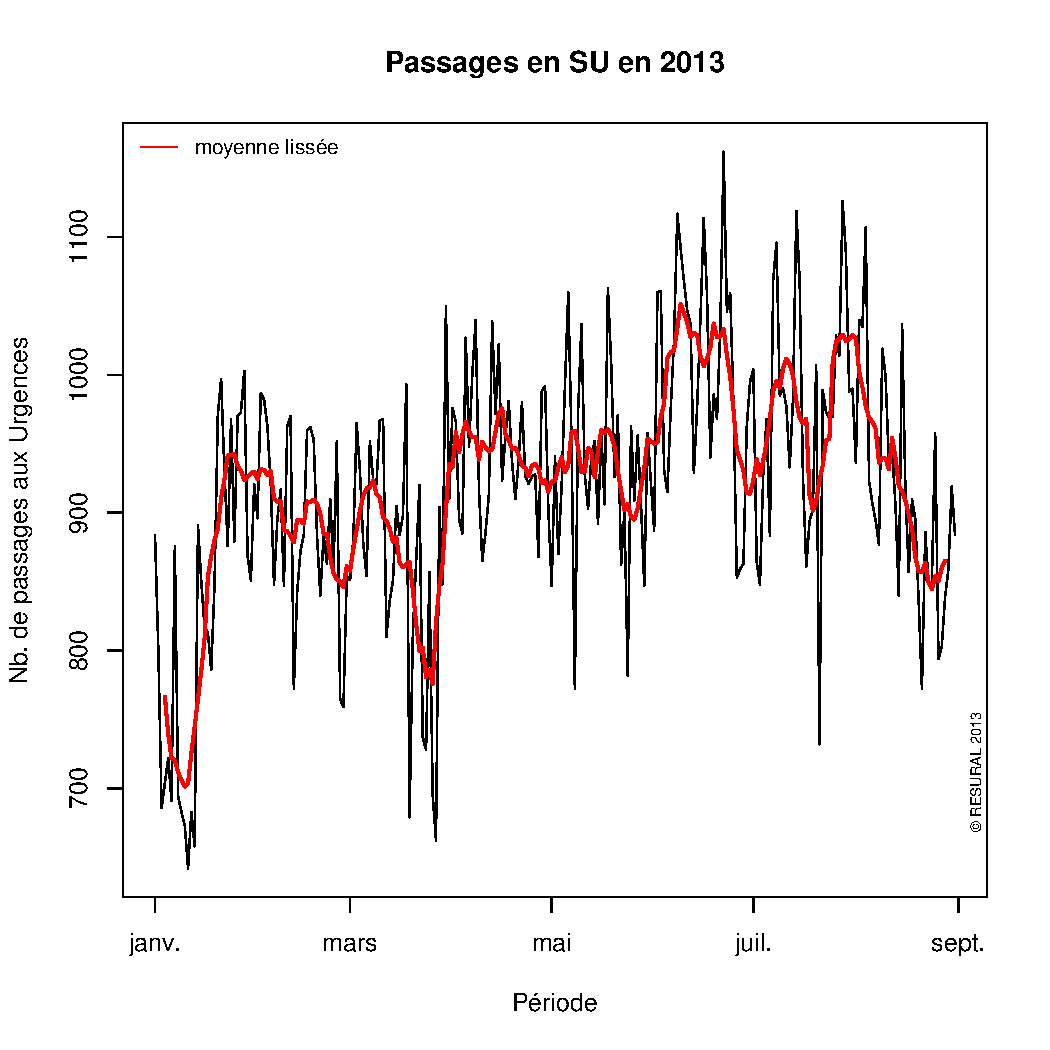
\includegraphics[width=\maxwidth]{figure/activite_plot} 

\end{knitrout}

% Variante avec *xts*
\begin{knitrout}
\definecolor{shadecolor}{rgb}{0.969, 0.969, 0.969}\color{fgcolor}
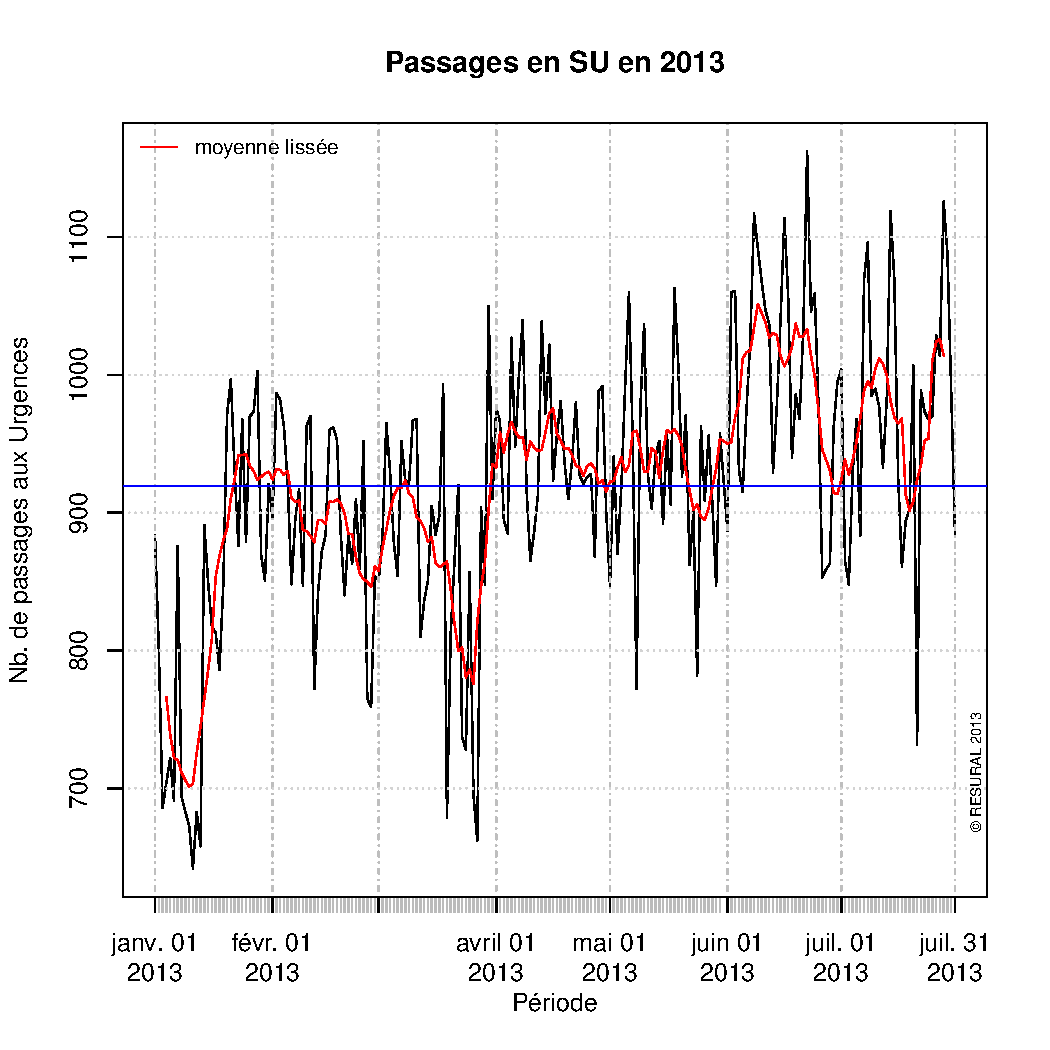
\includegraphics[width=\maxwidth]{figure/activite_plot2} 

\end{knitrout}


\subsection*{En valeur absolue}
\begin{knitrout}
\definecolor{shadecolor}{rgb}{0.969, 0.969, 0.969}\color{fgcolor}\begin{kframe}
\begin{alltt}
t <- \hlkwd{tapply}(\hlkwd{as.Date}(d1$ENTREE), d1$FINESS, length)
t
\end{alltt}
\begin{verbatim}
##   3Fr   Alk   Col   Dia   Geb   Hag   Hus   Mul   Odi   Sel   Wis   Sav 
##  9382  3784 38722 17150  8852 20531 22438 31533 15193 17496  7431   590
\end{verbatim}
\end{kframe}
\end{knitrout}


\subsection*{En pourcentage}
\begin{knitrout}
\definecolor{shadecolor}{rgb}{0.969, 0.969, 0.969}\color{fgcolor}\begin{kframe}
\begin{alltt}
\hlkwd{round}(\hlkwd{prop.table}(t) * 100, 2)
\end{alltt}
\begin{verbatim}
##   3Fr   Alk   Col   Dia   Geb   Hag   Hus   Mul   Odi   Sel   Wis   Sav 
##  4.86  1.96 20.05  8.88  4.58 10.63 11.62 16.33  7.87  9.06  3.85  0.31
\end{verbatim}
\end{kframe}
\end{knitrout}


\subsection*{Taux de recours aux urgences}
\begin{knitrout}
\definecolor{shadecolor}{rgb}{0.969, 0.969, 0.969}\color{fgcolor}\begin{kframe}
\begin{alltt}
tru2011_lorraine <- 0.2345
tru_estime <- pop.als.2010.totale * tru2011_lorraine
\hlcom{# tru2013_alsace<-round(length(e)*100/pop.als.2010.totale,2)}
tru2013_alsace <- \hlkwd{round}(\hlkwd{nrow}(d1) * 100/pop.als.2010.totale, 2)

\hlkwd{print}(tru_estime)
\end{alltt}
\begin{verbatim}
## [1] 441062
\end{verbatim}
\end{kframe}
\end{knitrout}

Le taux de recours aux urgences \index{taux de recours aux urgences} (TRU) \index{TRU} est défini comme le nombre total de passages aux urgences, rapporté à la population de la région (INSEE 1er janvier 2010). En Lorraine, ce taux est estimé à 23,45\% en 2010 (\cite{2,3}). En supposant que la population alsacienne se comprte comme la population lorraine, le nombre de passages aux urgences devrait s'établir à \ensuremath{4.4106\times 10^{5}}.

Le TRU 2013 estimé en Alsace à partir des RPU transmis est de 10.27\%.

\subsection*{Activité par mois}
%------------------------------
\begin{knitrout}
\definecolor{shadecolor}{rgb}{0.969, 0.969, 0.969}\color{fgcolor}\begin{kframe}
\begin{alltt}
m <- \hlkwd{month}(d1$ENTREE, label = TRUE)
\hlkwd{table}(m)
\end{alltt}
\begin{verbatim}
## m
##   Jan   Feb   Mar   Apr   May   Jun   Jul   Aug   Sep   Oct   Nov   Dec 
## 25609 25004 26937 28428 27899 30038 29187     0     0     0     0     0
\end{verbatim}
\begin{alltt}
\hlkwd{barplot}(\hlkwd{table}(m), ylab = \hlstr{"nombre"}, xlab = \hlstr{"mois"}, main = \hlstr{"2013 - Nombre de RPU par mois"}, 
    names.arg = \hlkwd{c}(\hlstr{"Jan"}, \hlstr{"Fev"}, \hlstr{"Mar"}, \hlstr{"Avr"}, \hlstr{"Mai"}, \hlstr{"Jui"}, \hlstr{"Jul"}, \hlstr{"Aou"}, \hlstr{"Sep"}, 
        \hlstr{"Oct"}, \hlstr{"Nov"}, \hlstr{"Dec"}), las = 2)
\end{alltt}
\end{kframe}
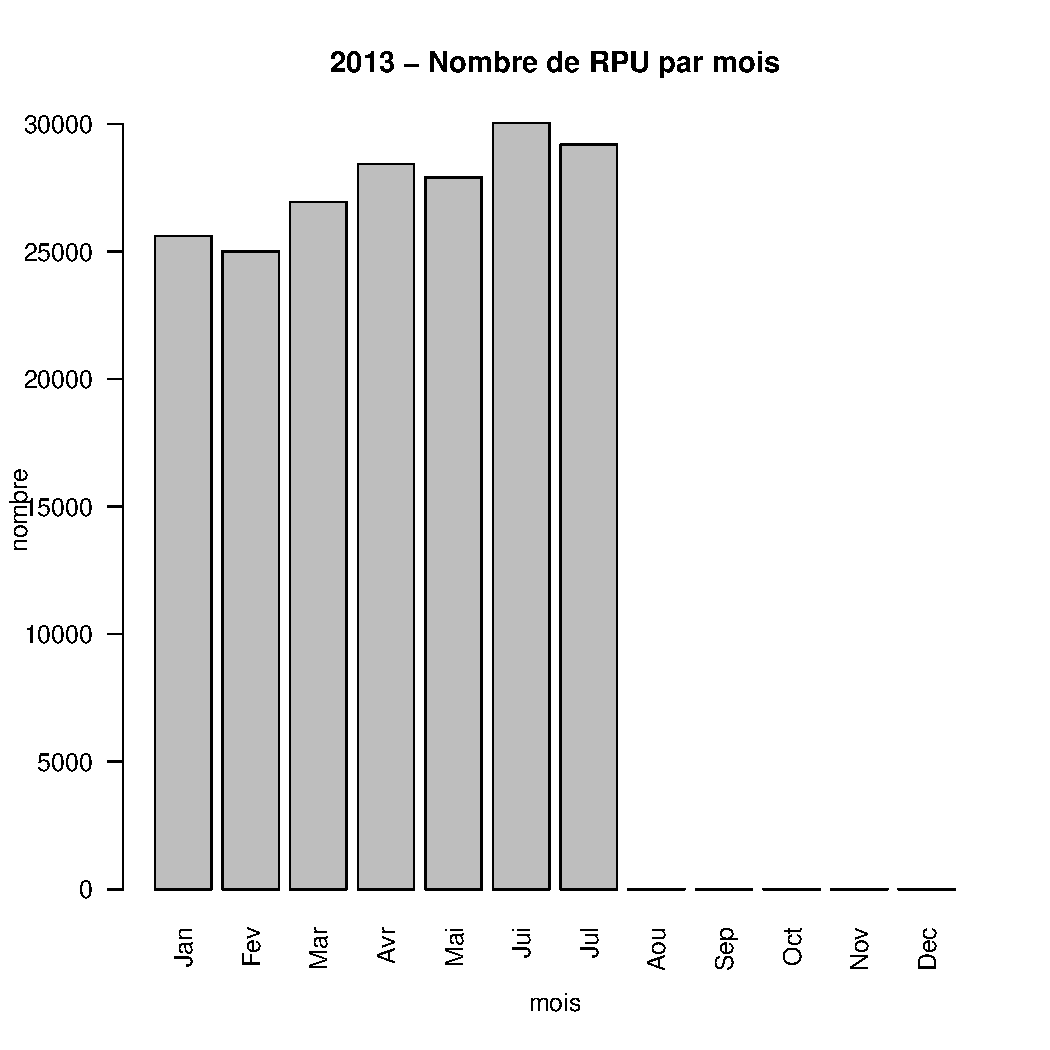
\includegraphics[width=\maxwidth]{figure/parmois} 

\end{knitrout}


\subsection*{Activité par semaine}

% latex table generated in R 2.15.1 by xtable 1.7-1 package
% Sun Aug 18 17:23:49 2013
\begin{table}[ht]
\centering
\begin{tabular}{rr}
  \hline
 & m \\ 
  \hline
1 & 4488 \\ 
  2 & 4909 \\ 
  3 & 5975 \\ 
  4 & 6593 \\ 
  5 & 6509 \\ 
  6 & 6354 \\ 
  7 & 6262 \\ 
  8 & 6193 \\ 
  9 & 6028 \\ 
  10 & 6426 \\ 
  11 & 6152 \\ 
  12 & 5735 \\ 
  13 & 5926 \\ 
  14 & 6698 \\ 
  15 & 6632 \\ 
  16 & 6667 \\ 
  17 & 6538 \\ 
  18 & 6462 \\ 
  19 & 6628 \\ 
  20 & 6720 \\ 
  21 & 6314 \\ 
  22 & 5615 \\ 
  23 & 7116 \\ 
  24 & 7213 \\ 
  25 & 7193 \\ 
  26 & 6569 \\ 
  27 & 6566 \\ 
  28 & 7083 \\ 
  29 & 6391 \\ 
  30 & 7069 \\ 
  31 & 2078 \\ 
   \hline
\end{tabular}
\caption[Activité par semaine]{Activité des SU par semaine en 2013} 
\label{act_sem}
\end{table}
% latex table generated in R 2.15.1 by xtable 1.7-1 package
% Sun Aug 18 17:23:49 2013
\begin{table}[ht]
\centering
\begin{tabular}{rrrrrrrrrrrrrrrrrrrrrrrrrrrrrrrr}
  \hline
 & 1 & 2 & 3 & 4 & 5 & 6 & 7 & 8 & 9 & 10 & 11 & 12 & 13 & 14 & 15 & 16 & 17 & 18 & 19 & 20 & 21 & 22 & 23 & 24 & 25 & 26 & 27 & 28 & 29 & 30 & 31 \\ 
  \hline
1 & 4488 & 4909 & 5975 & 6593 & 6509 & 6354 & 6262 & 6193 & 6028 & 6426 & 6152 & 5735 & 5926 & 6698 & 6632 & 6667 & 6538 & 6462 & 6628 & 6720 & 6314 & 5615 & 7116 & 7213 & 7193 & 6569 & 6566 & 7083 & 6391 & 7069 & 2078 \\ 
   \hline
\end{tabular}
\caption[Activité par semaine]{Activité des SU par semaine en 2013} 
\label{act_sem2}
\end{table}

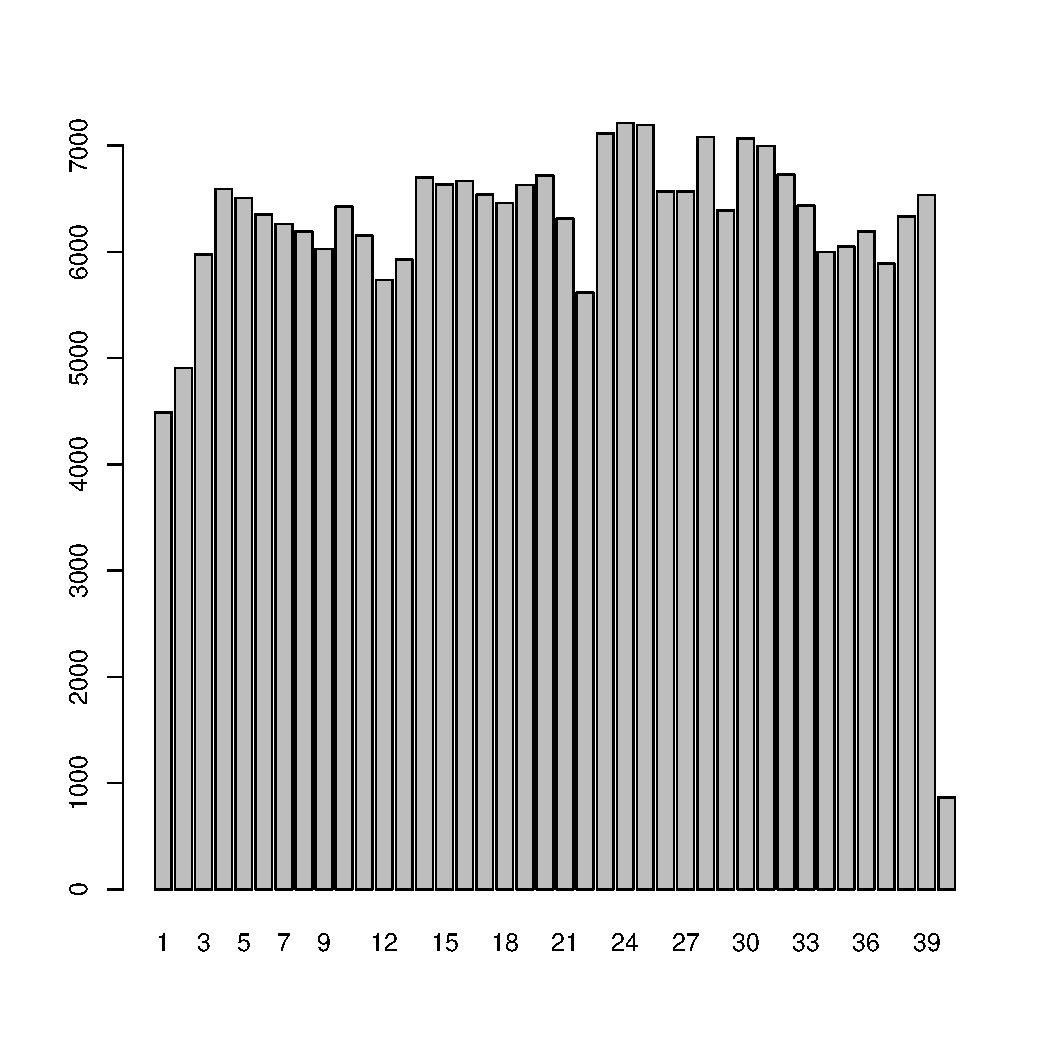
\includegraphics[width=\maxwidth]{figure/act_sem} 



\subsection*{Activité par jour de la semaine}
\begin{knitrout}
\definecolor{shadecolor}{rgb}{0.969, 0.969, 0.969}\color{fgcolor}\begin{kframe}
\begin{alltt}
m <- \hlkwd{wday}(d1$ENTREE, label = T)
\hlkwd{table}(m)
\end{alltt}
\begin{verbatim}
## m
##   Sun   Mon  Tues   Wed Thurs   Fri   Sat 
## 28591 29737 27681 25799 27050 26150 28094
\end{verbatim}
\begin{alltt}
\hlkwd{barplot}(\hlkwd{table}(m), names.arg = \hlkwd{c}(\hlstr{"Dim"}, \hlstr{"Lun"}, \hlstr{"Mar"}, \hlstr{"Mer"}, \hlstr{"Jeu"}, \hlstr{"Ven"}, \hlstr{"Sam"}))
\end{alltt}
\end{kframe}
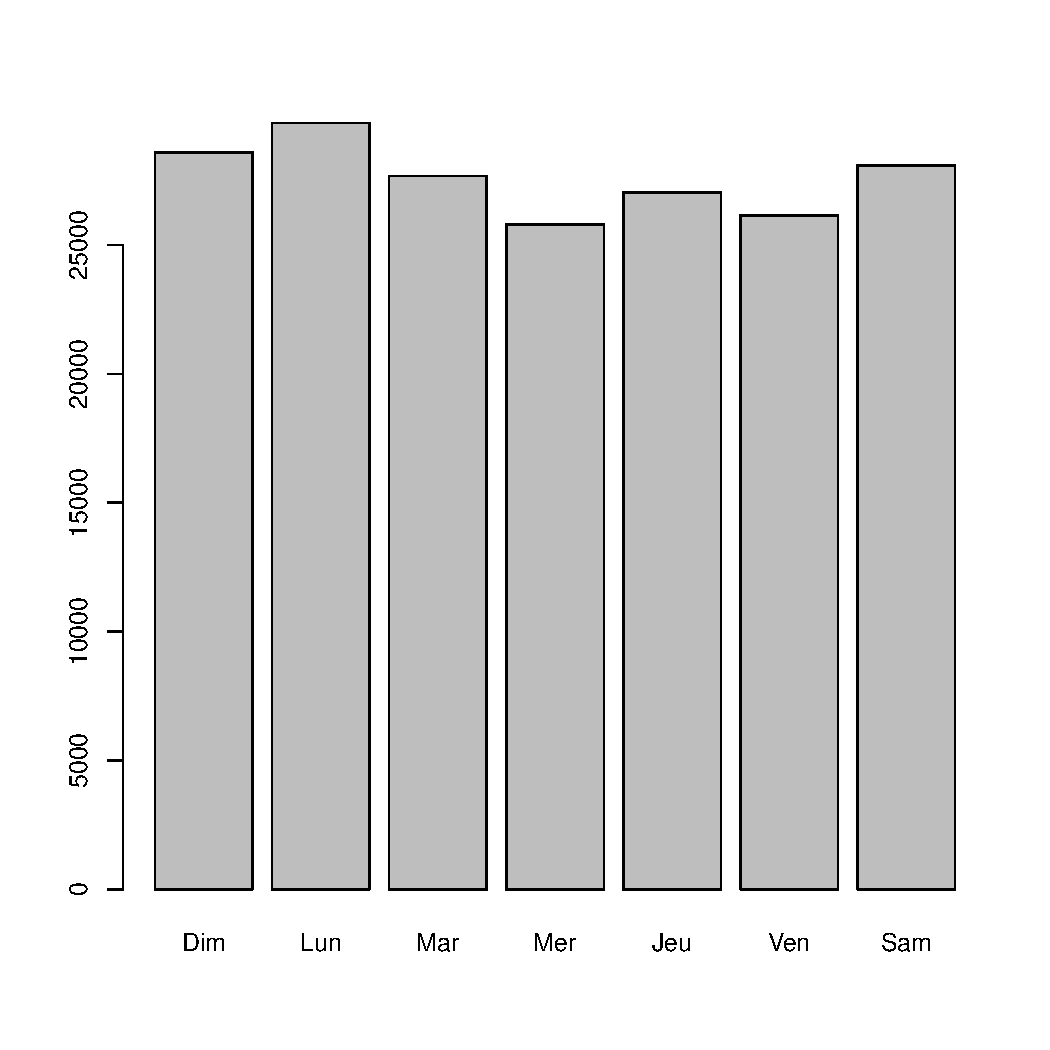
\includegraphics[width=\maxwidth]{figure/unnamed-chunk-17} 

\end{knitrout}


\subsection*{Activité horaire}
\begin{knitrout}
\definecolor{shadecolor}{rgb}{0.969, 0.969, 0.969}\color{fgcolor}\begin{kframe}
\begin{alltt}
h <- \hlkwd{hour}(d1$ENTREE)
t <- \hlkwd{table}(h)
\hlkwd{barplot}(\hlkwd{table}(h), xlab = \hlstr{"Heures de la journée"}, ylab = \hlstr{"nombre"}, main = \hlstr{"Répartition des RPU sur le nycthémère"})
\end{alltt}
\end{kframe}
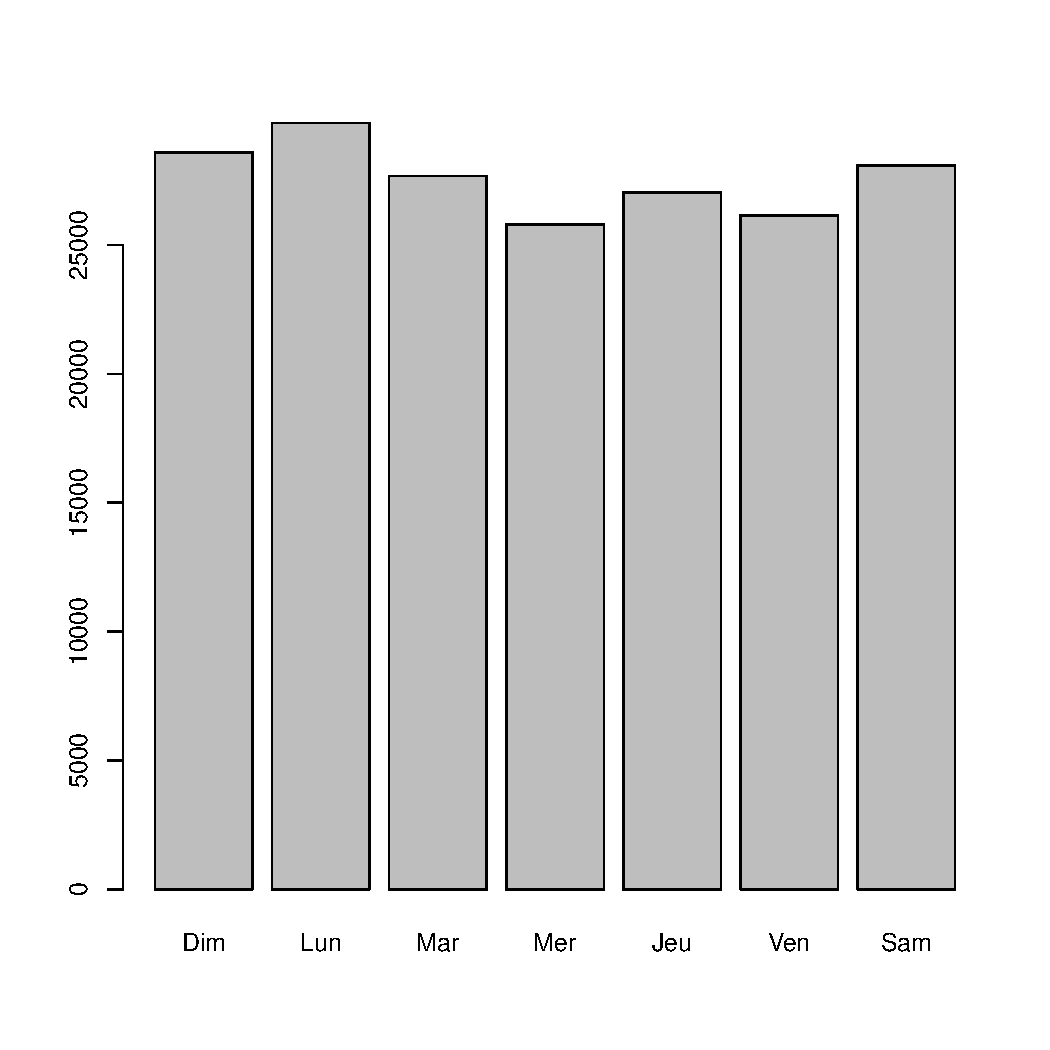
\includegraphics[width=\maxwidth]{figure/unnamed-chunk-18} 

\end{knitrout}


  


% \section*{Nombre total de passages par SU}
% \subsection*{En valeur absolue}
% \subsection*{En pourcentage}
% \subsection*{Taux de recours aux urgences}
% \subsection*{Activité par mois}
% \subsection*{Activité par jour de la semaine}
% \subsection*{Activité horaire}


% test2.Rnw

L'activité horaire des services d'urgence en Alsace est totalement superposable à celui de l'ensamble des SU (figure \ref{passage:als} page \pageref{passage:als}). L'activité diminue fortement en nuit profonde à partir de une heure du matin pour redémarrer vers 9 heures et s'intensifier progressivement en matinée. Après un premier pic en fin de matinée, la croissance reprend pour culminer vers 19 heures, puis décroître lentement jusqu'en fin de soirée.

Ce phénomène cyclique se répète tous les jours selon un profil immuable. La projection de ces données sur un graphique en radar représentant les 24 tranches horaires (figure \ref{radar:als} page \pageref{radar:als}) montre qu'il existe trois pics d'égale amplitude à 11, 15 et 19 heures. Ce point mérite d'être analysé car s'il se confirme, cela pourrait indiquer que le pointage de 11 heures permet d'avoir une prévision sur l'intensité de la fréquentation avant la garde du soir. On peut en rapprocher le fait que la médiane des passages se situe vers 14h, c'est à dire qu'au ointage de 15 heures on peut évaluer la quantité totale de patients qui vont se présenter dans les heures qui viennent.

%----------------------------------------------------------------------------- Summary
\begin{knitrout}
\definecolor{shadecolor}{rgb}{0.969, 0.969, 0.969}\color{fgcolor}\begin{kframe}
\begin{verbatim}
[1] "Résumé des horaires de passage:"
   Min. 1st Qu.  Median    Mean 3rd Qu.    Max. 
    0.0    10.0    14.0    13.9    18.0    23.0 
\end{verbatim}
\end{kframe}
\end{knitrout}


% latex table generated in R 2.15.1 by xtable 1.7-1 package
% Thu Jul 4 19:27:36 2013
\begin{table}[ht]
\centering
\begin{tabular}{rrrrrrr}
\hline
& Min. & Q1 & Médiane & Moyenne & Q3 & Max. \\
\hline
1 & 0.00 & 10.00 & 14.00 & 13.80 & 18.00 & 23.00 \\
\hline
\end{tabular}
\caption[titre court]{titre long}
\label{lab}
\end{table}


% latex table generated in R 2.15.1 by xtable 1.7-1 package
% Thu Jul 4 19:27:36 2013
\begin{table}[ht]
\centering
\begin{tabular}{rrrrrrr}
\hline
& moyenne & écart-type & médiane & min & max & n \\
\hline
1 & 13.82 & 5.54 & 14.00 & 0.00 & 23.00 & 105979.00 \\
\hline
\end{tabular}
\caption[Horaires de passage]{Horaires de passages au service des urgences en Alsace}
\label{hor:pass}
\end{table}

\input{../blah.gen}
%---------------------------------------------------------------------- HISTOGRAMME

\begin{figure}
\begin{center}
\begin{knitrout}
\definecolor{shadecolor}{rgb}{0.969, 0.969, 0.969}\color{fgcolor}
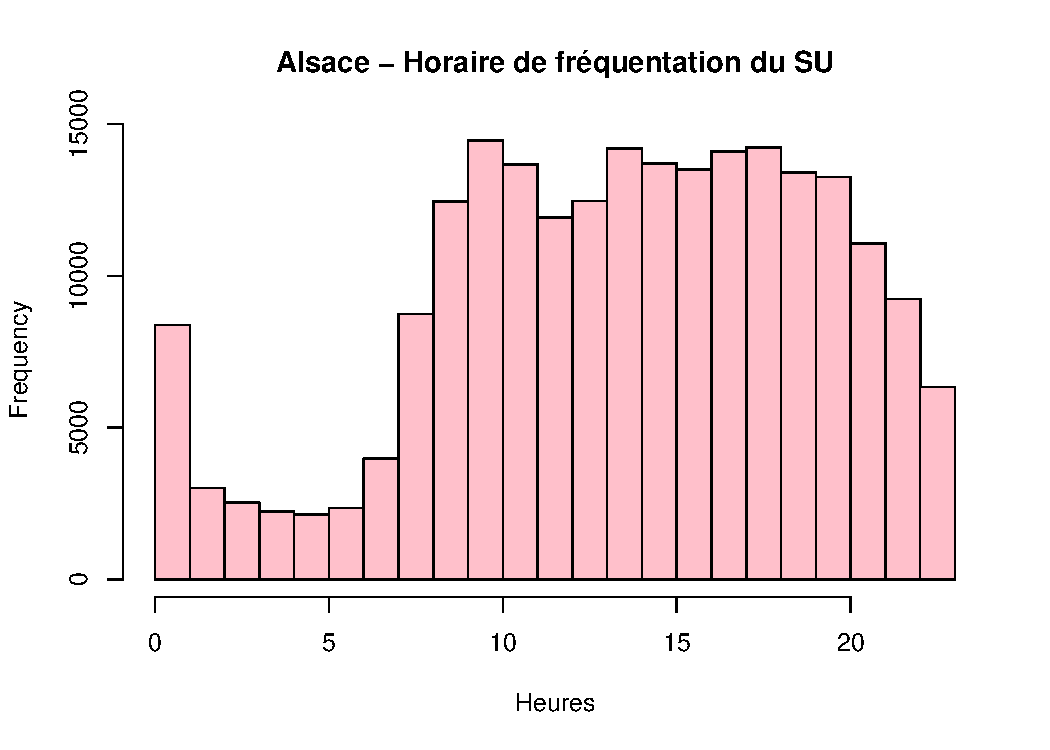
\includegraphics[width=\maxwidth]{figure/test23} 

\end{knitrout}

\end{center}
\caption{Horaires d'arrivée aux urgences en Alsace 2013}
\label{passage:als}
\end{figure}
%---------------------------------------------------------------------------- RADAR 1

\begin{figure}
\begin{center}
\begin{knitrout}
\definecolor{shadecolor}{rgb}{0.969, 0.969, 0.969}\color{fgcolor}
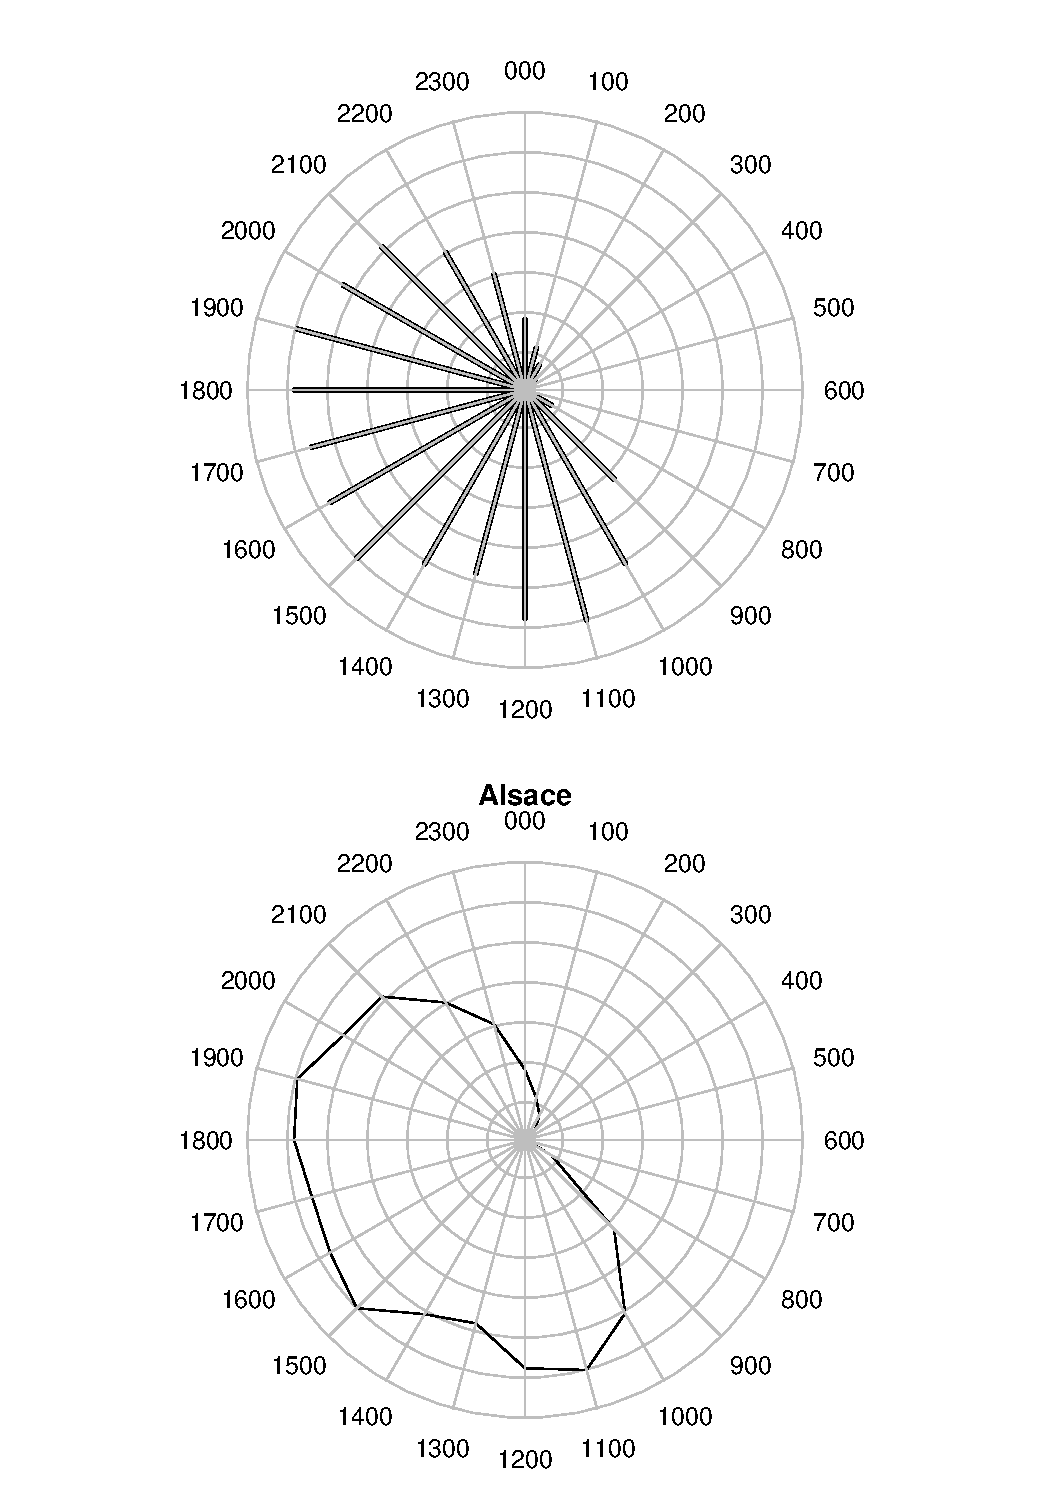
\includegraphics[width=\maxwidth]{figure/test25} 

\end{knitrout}

\end{center}
\caption{Horaires d'arrivée aux urgences en Alsace 2013}
\label{radar:als}
\end{figure}

%---------------------------------------------------------Radar HUS
\begin{figure}
\begin{center}
\begin{knitrout}
\definecolor{shadecolor}{rgb}{0.969, 0.969, 0.969}\color{fgcolor}
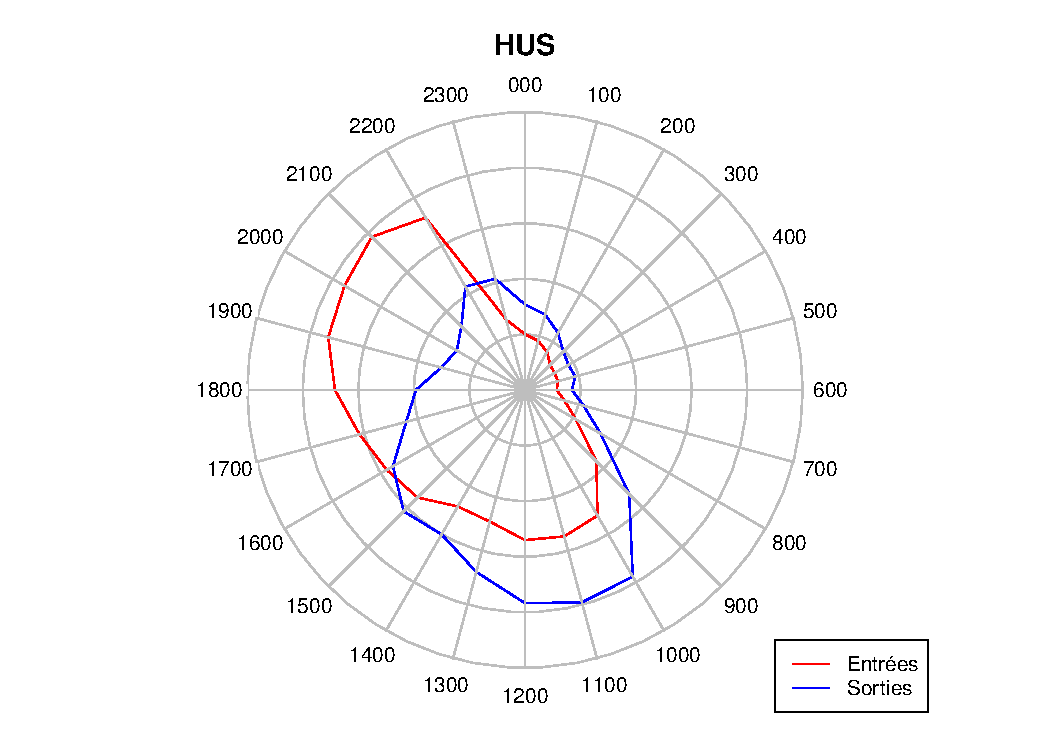
\includegraphics[width=\maxwidth]{figure/test2} 

\end{knitrout}

\end{center}
\caption{HUS: répartition des arrivées et départs aux urgences}
\label{passage:hus}
\end{figure}

%----------------------------------------------------------------
\begin{figure}
\begin{center}
\begin{knitrout}
\definecolor{shadecolor}{rgb}{0.969, 0.969, 0.969}\color{fgcolor}
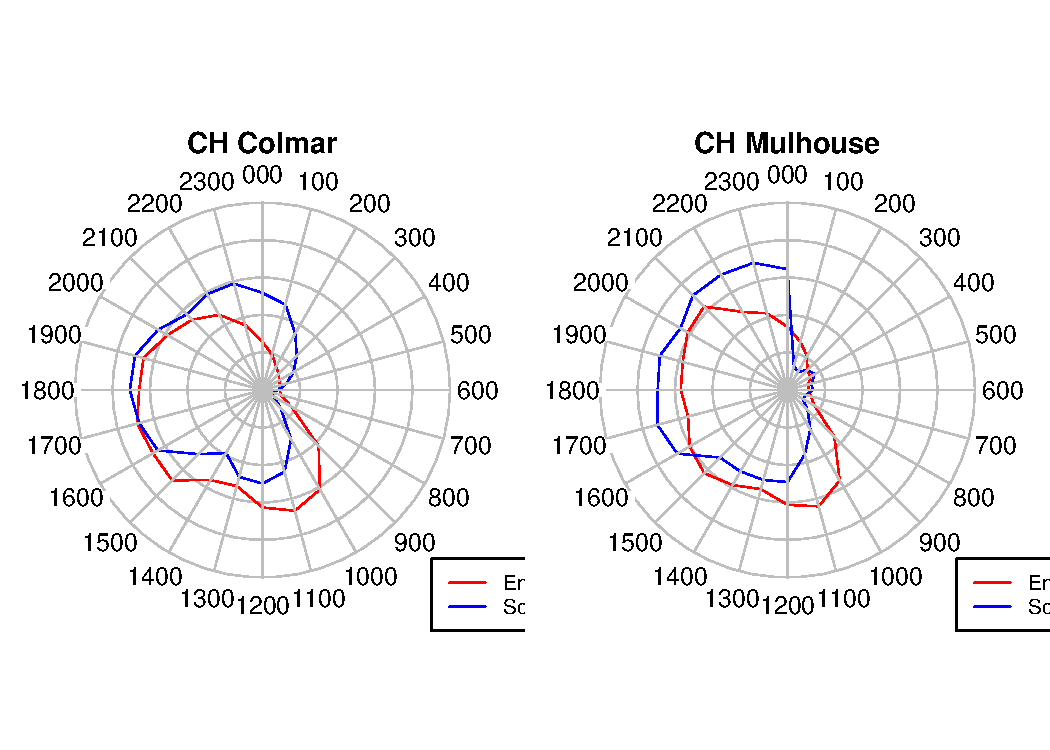
\includegraphics[width=\maxwidth]{figure/test22} 

\end{knitrout}

\end{center}
\caption{CH Colmar et Mulhouse: répartition des arrivées et départs aux urgences}
\label{passage:col}
\end{figure}



\subsection*{Passages par tranches d'âge}

\chapter{Modalité d'admission}

% modalites.Rnw
% modalités d'admission MODE_ENTREE

\index{Mode d'entrée}

\section*{Origine des patients}
% REMARQUE dans environ 300 dossiers du mois de juin, l'item transfert est écrit "transfe  rt" ce qui nécessite un recodage.

L'immense majorité des patients provient du domicile ou son équivalent. Une très faible part des passages aux urgences sont le fait de transferts d'autres établissements ou de mutations en provenance d'autres services du même établissement.


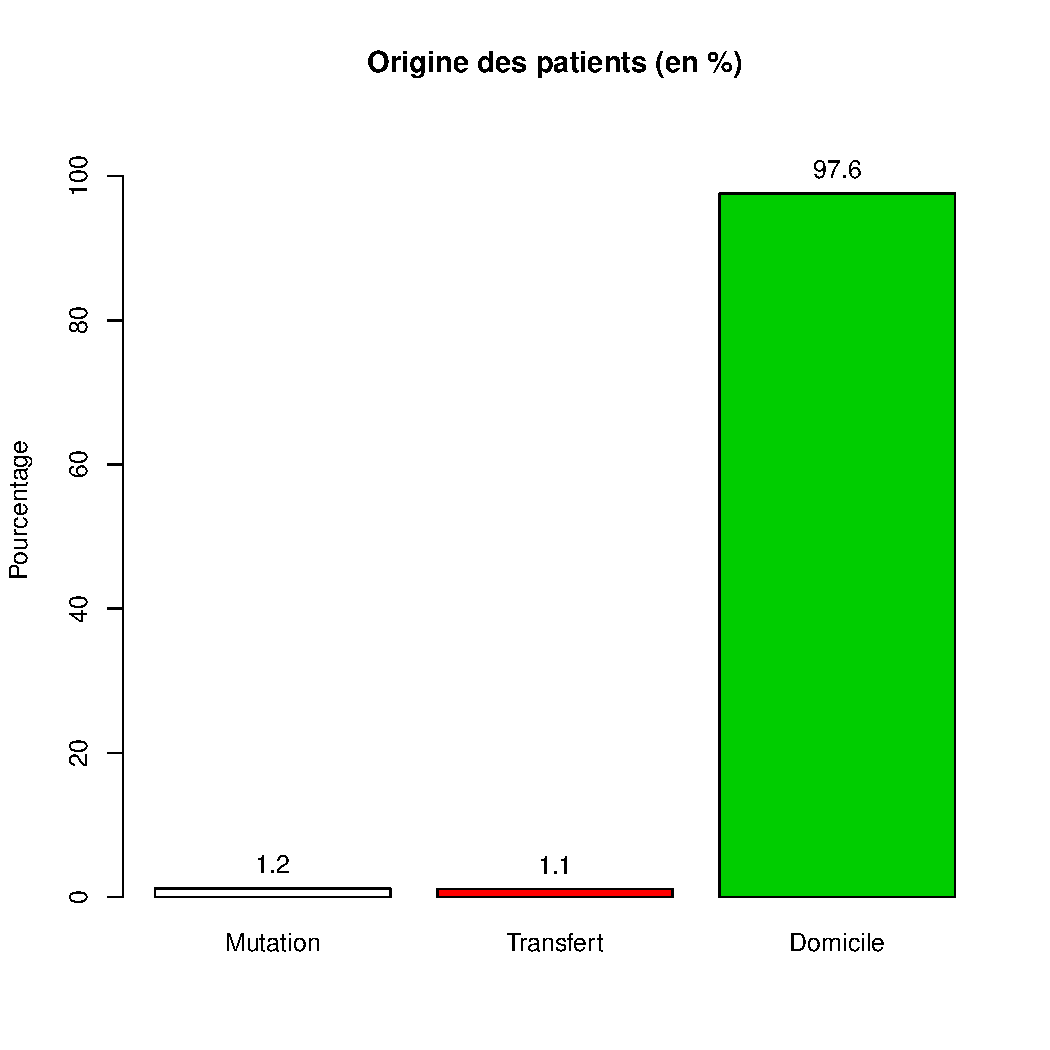
\includegraphics[width=\maxwidth]{figure/mode_entree} 
% latex table generated in R 2.15.1 by xtable 1.7-1 package
% Sun Aug 18 17:23:57 2013
\begin{table}[ht]
\centering
\begin{tabular}{rrrr}
  \hline
 & Frequency &   \%(NA+) &   \%(NA-) \\ 
  \hline
Mutation & 2167.00 & 1.10 & 1.30 \\ 
  Transfert & 1959.00 & 1.00 & 1.10 \\ 
  Domicile & 167773.00 & 86.90 & 97.60 \\ 
  NA's & 21203.00 & 11.00 & 0.00 \\ 
    Total & 193102.00 & 100.00 & 100.00 \\ 
   \hline
\end{tabular}
\caption[Origine des patients]{Origine des patients. Les deux colonnes de droite mesurent l'origine (en pourcentage) selon que l'on prenne en compte ou non les valeurs manquantes. } 
\label{origine}
\end{table}



Dans 11 \% des cas, l'origine du patient n'est pas précisée.

\section*{Mode de transport}
\index{Mode de transport}

La grande majorité des patients arrivent aux urgences par leurs propres moyens (PERSO). Lorsqu'ils font appel à un tiers, il s'agit le plus souvent d'une ambulance privée (AMBU), puis du SDIS (AMBU). Les transports par un vecteur médicalisé (SMUR) ou héliporté (HELI) sont rares. Enfin l'utilisation des forces de l'ordre (FO) comme moyen de transport reste marginale.


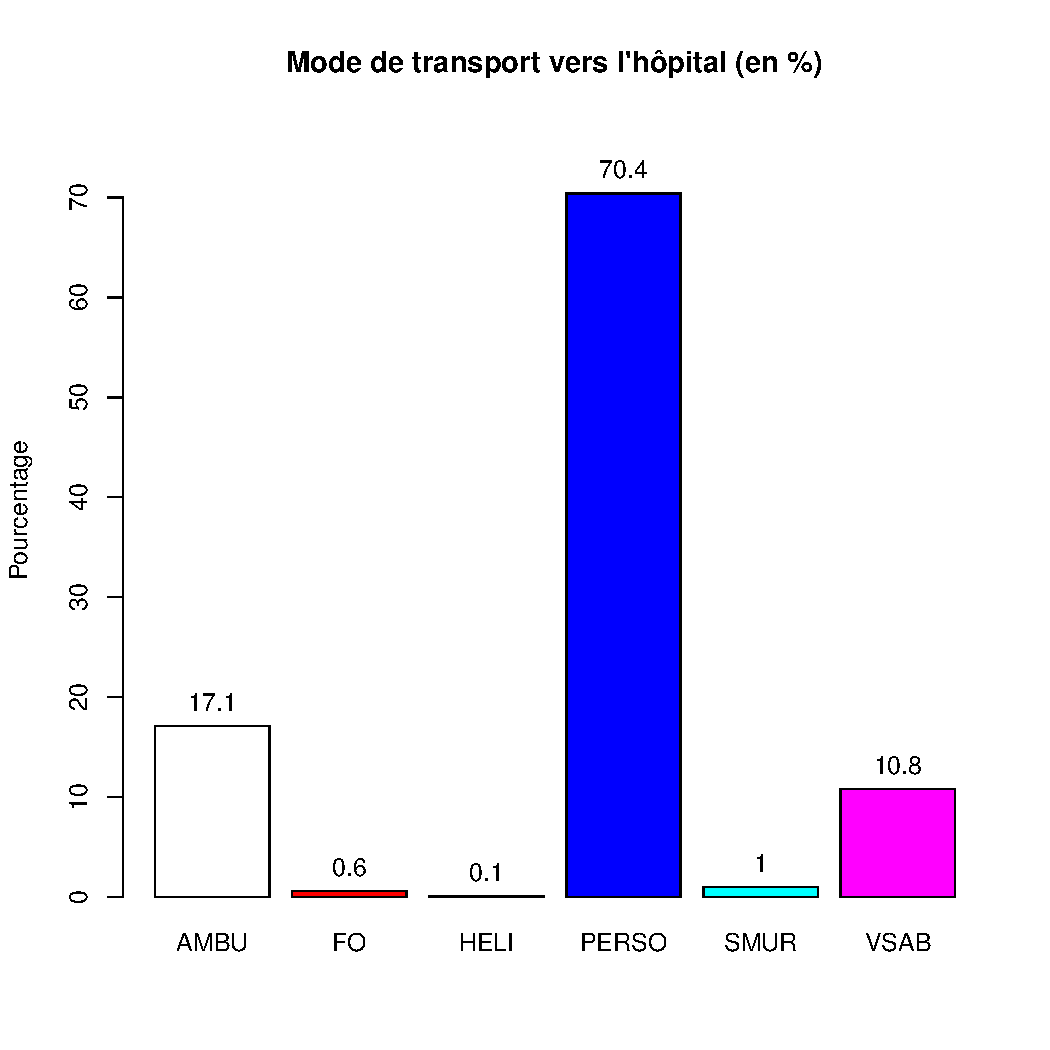
\includegraphics[width=\maxwidth]{figure/transport} 
% latex table generated in R 2.15.1 by xtable 1.7-1 package
% Sun Aug 18 17:23:57 2013
\begin{table}[ht]
\centering
\begin{tabular}{rrrr}
  \hline
 & Frequency &   \%(NA+) &   \%(NA-) \\ 
  \hline
AMBU & 26860.00 & 13.90 & 17.40 \\ 
  FO & 845.00 & 0.40 & 0.50 \\ 
  HELI & 113.00 & 0.10 & 0.10 \\ 
  PERSO & 108184.00 & 56.00 & 70.10 \\ 
  SMUR & 1653.00 & 0.90 & 1.10 \\ 
  VSAB & 16682.00 & 8.60 & 10.80 \\ 
  NA's & 38765.00 & 20.10 & 0.00 \\ 
    Total & 193102.00 & 100.00 & 100.00 \\ 
   \hline
\end{tabular}
\caption[Moyens de transport]{Moyens de transport utilisés pour se rendre à l'hôpital. Les deux colonnes de droite mesurent la fréquence du moyen utilise (en pourcentage) selon que l'on prenne en compte ou non les valeurs manquantes. } 
\label{transport}
\end{table}



Dans 20.1 \% des cas, le moyen de transport utilisé par le patient pour rejoindre l'hôpial n'est pas précisé.

\section*{Origine géographique}



Les patients consultant aux urgences sont majoritairement issus de la région Alsace. Mais l'origine est très diverse, aussi bien en provenance des autres départements français qu'hors de France:
% \begin{itemize}
%   \item Alsace: cp_als (\Sexpr(round(cp_als*100/n,2) \%))
%   \item hors Alsace: cp_hals
%   \item dont hors de France: cp_monde
% \end{itemize}



\chapter{Durée de passage}
\section*{Selon l'heure}
\section*{Selon l'âge}
\section*{Selon le jour de la semaine}
\section*{Selon la structure}
\subsection*{Pourcentage de passages en moins de 4 heures par établissement}
\section*{Selon l'orientation}
\section*{Selon la gravité}

\chapter{Codage diagnostic}

\chapter{Modalités de sortie}

% sortie.Rnw

\subsection{Mode de sortie}
\index{mode de sortie}

Le RPU connaît trois mode de sortie des urgences:
\begin{enumerate}
  \item le décès
  \item le retour à domicile (ou ce qui en tient lieu)
  \item l'hospitalisation (mutation ou transfert)
\end{enumerate}

% Mode de SORTIE.png: 669x437 pixel, 72dpi, 23.60x15.42 cm, bb=0 0 669 437
 \begin{figure}[h]
 \centering
 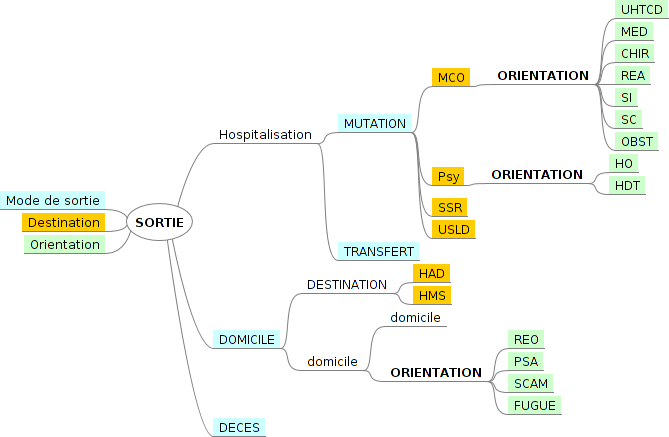
\includegraphics[width=9cm,height=7cm,bb=0 0 669 437]{figure/Mode de SORTIE.png}
 \caption{Modes de sortie}
\end{figure}

% latex table generated in R 2.15.1 by xtable 1.7-1 package
% Sun Aug 18 17:23:58 2013
\begin{table}[ht]
\centering
\begin{tabular}{|l|r|r|}
  \hline
 & n & \% \\ 
  \hline
Décès & 2 & 0.00 \\ 
  Domicile & 123148 & 63.77 \\ 
  Mutation & 38183 & 19.77 \\ 
  $<$NA$>$ & 29007 & 15.02 \\ 
  Transfert & 2762 & 1.43 \\ 
   \hline
\end{tabular}
\caption{Mode de sortie des urgences. <NA> est le nombre de non réponses à cet item} 
\label{tab.sortie}
\end{table}



\subsection{Orientation}
\index{orientation}

Le mode de sortie est affiné par la rubrique ORIENTATION avec la ventilation suivante:

\begin{itemize}
  \item NA:    Pas d'informations
  \item MCO:		Hospitalisation conventionnelle
  \item SSR:		Soins de suite et de réadaptation
  \item SLD:		Soins de longue durée
  \item PSY: 		Psychiatrie
  \item HAD:		Hospitalisation à domicile
  \item HMS:		Hébergement médico-social
\end{itemize}

On notera que le retour à domicile proprement dit ne figure pas parmi les items et cette modalité est implicite. On peut supposer que les NA's correspondent à cette modalité. Cependant une ambiguité demeure car les non réponses sont aussi représentées par ce symbole.

\begin{knitrout}
\definecolor{shadecolor}{rgb}{0.969, 0.969, 0.969}\color{fgcolor}\begin{kframe}
\begin{alltt}
\hlcom{# drop.levels permet d'éliminer le level 0 qui est nul}
a <- \hlkwd{drop.levels}(d1$ORIENTATION)
\hlkwd{summary}(a)
\end{alltt}
\begin{verbatim}
##   CHIR  FUGUE    HDT     HO    MED   OBST    PSA    REA    REO     SC 
##   4285    147     76     19   9790     60   1825    573    793    785 
##   SCAM     SI   UHCD   NA's 
##    280    788  19300 154381
\end{verbatim}
\begin{alltt}

\hlkwd{table}(a, useNA = \hlstr{"always"})
\end{alltt}
\begin{verbatim}
## a
##   CHIR  FUGUE    HDT     HO    MED   OBST    PSA    REA    REO     SC 
##   4285    147     76     19   9790     60   1825    573    793    785 
##   SCAM     SI   UHCD   <NA> 
##    280    788  19300 154381
\end{verbatim}
\begin{alltt}

\hlkwd{table}(d1$DESTINATION, d1$GRAVITE)
\end{alltt}
\begin{verbatim}
##      
##           1     2     3     4     5     D     P
##   NA      0     0     0     0     0     0     0
##   MCO  1552 15713 15628  1653   404     6    93
##   SSR     0    15    16     2     0     0     0
##   SLD     0     4     2     2     0     0     0
##   PSY    31   161   107    10     5     0   369
##   HAD     0     1     0     0     0     0     0
##   HMS     3    12     2     0     0     0     0
\end{verbatim}
\end{kframe}
\end{knitrout}


\subsection{Destination}
\index{destination}
% latex table generated in R 2.15.1 by xtable 1.7-1 package
% Sun Aug 18 17:23:58 2013
\begin{table}[ht]
\centering
\begin{tabular}{rr}
  \hline
 & \% \\ 
  \hline
HAD & 0.00 \\ 
  HMS & 0.04 \\ 
  MCO & 98.13 \\ 
  PSY & 1.72 \\ 
  SLD & 0.02 \\ 
  SSR & 0.08 \\ 
   \hline
\end{tabular}
\caption{Destination des patients non rentrés à domicile après leur passage aux urgences} 
\label{tab.dest.hosp}
\end{table}
% latex table generated in R 2.15.1 by xtable 1.7-1 package
% Sun Aug 18 17:23:58 2013
\begin{table}[ht]
\centering
\begin{tabular}{rr}
  \hline
 & \% \\ 
  \hline
DOM & 78.83 \\ 
  HAD & 0.00 \\ 
  HMS & 0.01 \\ 
  MCO & 20.78 \\ 
  PSY & 0.36 \\ 
  SLD & 0.00 \\ 
  SSR & 0.02 \\ 
   \hline
\end{tabular}
\caption{Devenir des patients à la sortie des urgences. DOM représentent ceux qui sont repartis vers leur domicile ou ce qui en tient lieu (sous l'hypothèse que toutes les non réponses correspondent à un retour à domicile).} 
\label{tab.dest}
\end{table}



\subsection{Incohérences}
\ref{sortie:erreurs}
On isole le groupe "mode de sortie = domicile) et on relève les résultats de l'item "orientation":
\begin{knitrout}
\definecolor{shadecolor}{rgb}{0.969, 0.969, 0.969}\color{fgcolor}\begin{kframe}
\begin{alltt}
a <- d1[d1$MODE_SORTIE == \hlstr{"Domicile"}, ]
\hlkwd{summary}(\hlkwd{as.factor}(a$ORIENTATION))
\end{alltt}
\begin{verbatim}
##   CHIR  FUGUE    HDT     HO    MED   OBST    PSA    REA    REO     SC 
##     73    146      9      1     48      1   1791      6    774      2 
##   SCAM     SI   UHCD   NA's 
##    280     21    141 148862
\end{verbatim}
\begin{alltt}
t <- \hlkwd{table}(\hlkwd{as.factor}(a$ORIENTATION))
\hlkwd{round}(\hlkwd{prop.table}(t) * 100, 2)
\end{alltt}
\begin{verbatim}
## 
##  CHIR FUGUE   HDT    HO   MED  OBST   PSA   REA   REO    SC  SCAM    SI 
##  2.22  4.43  0.27  0.03  1.46  0.03 54.39  0.18 23.50  0.06  8.50  0.64 
##  UHCD 
##  4.28
\end{verbatim}
\begin{alltt}
\hlkwd{tab1}(\hlkwd{as.factor}(a$ORIENTATION), sort.group = \hlstr{"decreasing"}, horiz = TRUE, cex.names = 0.8, 
    xlab = \hlstr{""}, main = \hlstr{"Orientation des patients non hospitalisés"}, missing = F)
\end{alltt}
\end{kframe}
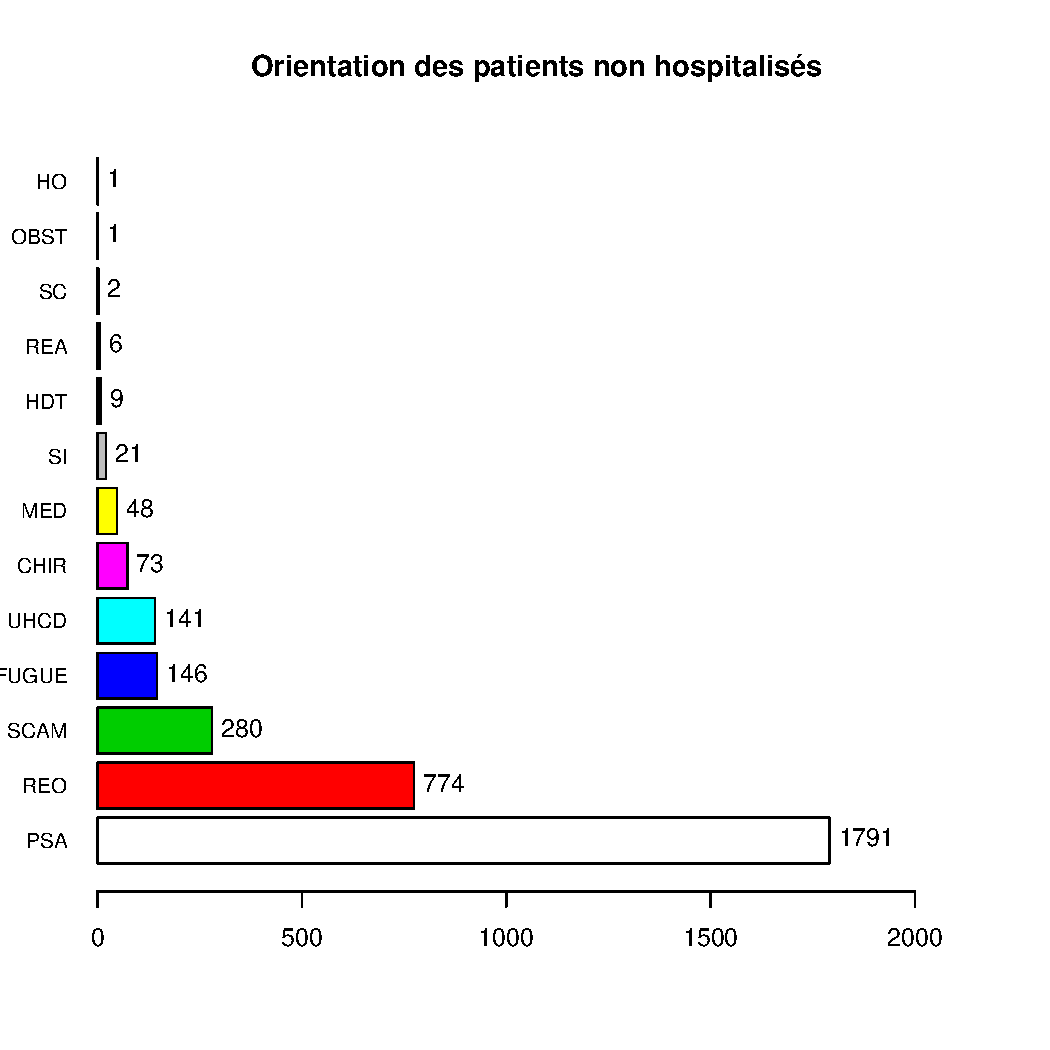
\includegraphics[width=\maxwidth]{figure/fausses_sorties} 
\begin{kframe}\begin{verbatim}
## as.factor(a$ORIENTATION) :  
##         Frequency   %(NA+)   %(NA-)
## NA's       148862     97.8      0.0
## PSA          1791      1.2     54.4
## REO           774      0.5     23.5
## SCAM          280      0.2      8.5
## FUGUE         146      0.1      4.4
## UHCD          141      0.1      4.3
## CHIR           73      0.0      2.2
## MED            48      0.0      1.5
## SI             21      0.0      0.6
## HDT             9      0.0      0.3
## REA             6      0.0      0.2
## SC              2      0.0      0.1
## HO              1      0.0      0.0
## OBST            1      0.0      0.0
##   Total    152155    100.0    100.0
\end{verbatim}
\end{kframe}
\end{knitrout}

Certaines orientations sont incompatibles avec une non hospitalisation:
\begin{itemize}
  \item HO
  \item Obstétrique
  \item Soins continus, soins intensifs et réanimation
  \item UHCD, médecine et chirurgie
  
\end{itemize}




\chapter{Modalités d'orientation}

\chapter{Courbes d'activité régionale}
\section*{Variation du nombre total de passages journaliers}
\section*{Variation du pourcentage journalier de retour à domicile}

%===================================================================== PARTIE 3
\part{Activité par service d'urgence}

\chapter{SAU des Hôpitaux universitaires}

% SuHus.Rnw
% Activité des SU des HUS
Les Hôpitaux universitaires de Strasbourg ont une offre étendue en matière d'urgences et seuleument certaines activités génèrent des RPU.
On compte:
\begin{enumerate}
  \item SU adulte du NHC
  \item SU adulte de HTP
  \item SU pédiatrique de HTP
  \item SU SOS mains (CCOM)
  \item SU Gynéco-obstétrique à HTP
\end{enumerate}
Auxquels il faut rajouter les services assurant un accueil des urgences 24h/24h et qui ne transitent pas par les SU. Ce sont les correspondants privilégiés du SAMU 67 et des transporteurs sanitaires (ASSU, VSAV, SMUR):
\begin{enumerate}
  \item Réanimations médicales de HTP et NHC
  \item Réanimations chirurgicales de HTP et NHC
  \item Réanimation pédiatrique polyvalente de HTP
  \item Unité neuro-vasculaire (HTP)
  \item SI cardio-vasculaire (NHC)
\end{enumerate}

\section{Activité globale}




Entre le 2013-01-01 00:11:00 et le 2013-07-30 23:55:00, \np{22438} RPU ont été transmis, alors que \np{41561} dossiers ont été déclarés au serveur régional. 
1, 1, 1, 1, 1



%===================================================================== PARTIE 4
\part{Activité des SAMU d'Alsace}

\chapter{Test un}

%\SweaveOpts{concordance=TRUE}
\begin{itemize}
  \item test2.Rnw exemple de graphiques avec label
\end{itemize}

\begin{knitrout}
\definecolor{shadecolor}{rgb}{0.969, 0.969, 0.969}\color{fgcolor}\begin{kframe}
\begin{alltt}
n <- \hlkwd{dim}(d1)
\hlkwd{print}(n)
\end{alltt}
\begin{verbatim}
## [1] 193102     20
\end{verbatim}
\begin{alltt}
\hlkwd{names}(d1)
\end{alltt}
\begin{verbatim}
##  [1] "id"            "CODE_POSTAL"   "COMMUNE"       "DESTINATION"  
##  [5] "DP"            "ENTREE"        "EXTRACT"       "FINESS"       
##  [9] "GRAVITE"       "MODE_ENTREE"   "MODE_SORTIE"   "MOTIF"        
## [13] "NAISSANCE"     "ORIENTATION"   "PROVENANCE"    "SEXE"         
## [17] "SORTIE"        "TRANSPORT"     "TRANSPORT_PEC" "AGE"
\end{verbatim}
\end{kframe}
\end{knitrout}



\chapter{test deux}
\begin{knitrout}
\definecolor{shadecolor}{rgb}{0.969, 0.969, 0.969}\color{fgcolor}\begin{kframe}
\begin{alltt}

\hlkwd{str}(d1)
\end{alltt}
\begin{verbatim}
## 'data.frame':	193102 obs. of  20 variables:
##  $ id           : chr  "2c9d83843bf5e01d013bf5e985d20225" "2c9d83843bf5e01d013bf5e986950226" "2c9d83843bf5e01d013bf5e987620227" "2c9d83843bf5e01d013bf5e988060228" ...
##  $ CODE_POSTAL  : Factor w/ 2116 levels "00000","00159",..: 706 706 706 706 706 701 818 706 706 706 ...
##  $ COMMUNE      : Factor w/ 4344 levels "00","01257 DRESDEN ALLEMAGNE",..: 2184 2184 2184 2184 741 2048 2033 2184 2184 2184 ...
##  $ DESTINATION  : Factor w/ 7 levels "NA","MCO","SSR",..: NA NA NA NA NA NA 2 NA 2 NA ...
##  $ DP           : chr  "R104" "J038" "S617" "M485" ...
##  $ ENTREE       : chr  "2013-01-01 00:04:00" "2013-01-01 00:16:00" "2013-01-01 00:26:00" "2013-01-01 00:32:00" ...
##  $ EXTRACT      : chr  "2013-01-01 05:37:00" "2013-01-01 05:37:00" "2013-01-01 05:37:00" "2013-01-01 05:37:00" ...
##  $ FINESS       : Factor w/ 12 levels "3Fr","Alk","Col",..: 10 10 10 10 10 10 10 10 10 10 ...
##  $ GRAVITE      : Factor w/ 7 levels "1","2","3","4",..: 2 2 3 2 2 1 3 2 2 2 ...
##  $ MODE_ENTREE  : Factor w/ 5 levels "NA","Mutation",..: 4 4 4 4 4 4 4 4 4 4 ...
##  $ MODE_SORTIE  : Factor w/ 5 levels "NA","Mutation",..: 4 4 4 4 4 4 2 4 2 4 ...
##  $ MOTIF        : chr  "GASTRO04" "DIVERS23" "TRAUMATO10" "TRAUMATO02" ...
##  $ NAISSANCE    : chr  "1960-04-08 00:00:00" "1986-03-05 00:00:00" "1971-12-22 00:00:00" "1927-04-27 00:00:00" ...
##  $ ORIENTATION  : Factor w/ 13 levels "CHIR","FUGUE",..: NA NA NA NA NA NA 5 NA 5 NA ...
##  $ PROVENANCE   : Factor w/ 7 levels "NA","MCO","SSR",..: 6 6 6 6 6 6 6 6 6 6 ...
##  $ SEXE         : Factor w/ 3 levels "F","I","M": 3 3 3 1 3 3 1 1 1 1 ...
##  $ SORTIE       : chr  "2013-01-01 02:38:00" "2013-01-01 00:38:00" "2013-01-01 02:07:00" "2013-01-01 01:52:00" ...
##  $ TRANSPORT    : Factor w/ 6 levels "AMBU","FO","HELI",..: 4 4 4 1 4 4 6 6 4 4 ...
##  $ TRANSPORT_PEC: Factor w/ 3 levels "AUCUN","MED",..: 1 1 1 3 1 1 2 2 1 1 ...
##  $ AGE          : num  52 26 41 85 39 9 79 50 46 18 ...
\end{verbatim}
\begin{alltt}
\hlkwd{summary}(d1)
\end{alltt}
\begin{verbatim}
##       id             CODE_POSTAL           COMMUNE        DESTINATION    
##  Length:193102      68000  : 13531   MULHOUSE  : 22610   MCO    : 40127  
##  Class :character   68200  : 11867   STRASBOURG: 20105   PSY    :   703  
##  Mode  :character   68100  : 10798   COLMAR    : 13527   SSR    :    33  
##                     67100  :  9169   HAGUENAU  :  4028   HMS    :    18  
##                     67000  :  6454   SELESTAT  :  3654   SLD    :     8  
##                     67600  :  5430   (Other)   :129174   (Other):     1  
##                     (Other):135853   NA's      :     4   NA's   :152212  
##       DP               ENTREE            EXTRACT              FINESS     
##  Length:193102      Length:193102      Length:193102      Col    :38722  
##  Class :character   Class :character   Class :character   Mul    :31533  
##  Mode  :character   Mode  :character   Mode  :character   Hus    :22438  
##                                                           Hag    :20531  
##                                                           Sel    :17496  
##                                                           Dia    :17150  
##                                                           (Other):45232  
##     GRAVITE            MODE_ENTREE        MODE_SORTIE    
##  2      :118082   NA         :     0   NA       :     0  
##  1      : 23288   Mutation   :  2167   Mutation : 38183  
##  3      : 22494   Transfert  :  1959   Transfert:  2762  
##  4      :  2084   Domicile   :167773   Domicile :123148  
##  P      :   843   Transfe  rt:     0   Décès    :     2  
##  (Other):   524   NA's       : 21203   NA's     : 29007  
##  NA's   : 25787                                          
##     MOTIF            NAISSANCE          ORIENTATION       PROVENANCE    
##  Length:193102      Length:193102      UHCD   : 19300   PEA    :107747  
##  Class :character   Class :character   MED    :  9790   PEO    : 16859  
##  Mode  :character   Mode  :character   CHIR   :  4285   MCO    :  4427  
##                                        PSA    :  1825   PSY    :    22  
##                                        REO    :   793   SSR    :    20  
##                                        (Other):  2728   (Other):    13  
##                                        NA's   :154381   NA's   : 64014  
##  SEXE          SORTIE          TRANSPORT      TRANSPORT_PEC   
##  F: 91478   Length:193102      AMBU : 26860   AUCUN  :137702  
##  I:     3   Class :character   FO   :   845   MED    :  3943  
##  M:101621   Mode  :character   HELI :   113   PARAMED:  4186  
##                                PERSO:108184   NA's   : 47271  
##                                SMUR :  1653                   
##                                VSAB : 16682                   
##                                NA's : 38765                   
##       AGE       
##  Min.   :  0.0  
##  1st Qu.: 18.0  
##  Median : 38.0  
##  Mean   : 40.4  
##  3rd Qu.: 61.0  
##  Max.   :112.0  
##  NA's   :6
\end{verbatim}
\end{kframe}
\end{knitrout}


\index{test}
\index{Eclipse@Eclipse!solaire}
\index{Orbite!périgée@périgée}
test biblio \cite{1}
%===================================================================== PARTIE 5
\part{Annexes}
\appendix
\chapter{Méthodologie}

% methodologie.Rnw

\section*{Taux de passage aux urgences}
  \begin{displaymath}
    \frac{\text{Nombre de passages déclarés par les SU}}{\text{Population globale d'Alsace}}
  \end{displaymath}

\section*{Taux de recours aux urgences}
\begin{displaymath}
    \frac{\text{Nombre de passages d' Alsace}}{\text{Population globale d'Alsace}}
  \end{displaymath}
Le Nombre de passages d' Alsace est la somme des passages dans les SU alsacien ET des passages de résidents alsacien dans des SU limitrophes.

\section*{Taux d'intervention régional}
\begin{displaymath}
    \frac{\text{Nombre de patients pris en charge par les SMUR d'Alsace quelque soit le code postal du lieu d'intervention}}{\text{Population globale d'Alsace}}
  \end{displaymath}

\section*{Taux de recours régional}
\begin{displaymath}
    \frac{\text{Nombre de patients pris en charge par un SMUR dont l'intervention a lieu sur le territoire régional }}{\text{Population globale d'Alsace}}
  \end{displaymath}

\section*{Rapport de masculinité ou sex-ratio}
\begin{displaymath}
    \frac{\text{Nombre d'Hommes}}{\text{Nombre de Femmes}} \times 100
\end{displaymath}

Une valeur supérieure à 1 indique qu'il y a plus d'hommes que de femmes.

\section*{Définition de la semaine}
La semaine est définie comme la péride complémentaire du week-end. La semaine s'étend du lundi $08:00$ heures au vendredi $19:59$.

\section*{Définition du Week-end}
L'offre de soins comme la fréquentation des SU n'est pas identique en coiurs de semaine et en fin de semaine. C'est pourquoi est introduite la notion temporelle de week-end.
Le week-end est défini comme la période allant du vendredi soir 20h au lundi matin 07h59.

\section*{Moyenne mobile}
Une moyenne mobile permet de lisser une série de valeurs, permettant de gommer des fluctuations temporelles. La moyenne mobile d'odre $7$ est très utilisée pour analyser les données temporelles. Elle permet notamment d'atténuer les pics de fréquentation des SU le week-end.
\begin{displaymath}
    \frac{\text{somme des passages 7 jours consécutifs}}{7}
\end{displaymath}
Les moyennes mobiles sont généralement présentées sous forme "glissante", c'est à dire sous la forme d'une succession de groupe de sept éléments, décalés d'une journée.

\section*{Pondération annuelle et mensuelle}
Le nombre de jour dans un mois est variable d'un mois à l'autre. Il en va de même pour le nombre de jours d'une année, où du nombre de répétitions d'un jour donné de la semaine.

\chapter{Glossaire}

% glossaire.Rnw

\glossary{AIT Accident (Vasculaire) Ischemique Transitoire}



\subsection*{AIT}
\index{AIT}
Accident (Vasculaire) Ischemique Transitoire

\subsection*{ANTARES}
\index{ANTARES}
Adaptation Nationale des Trasmissions Aux Risques Et Secours

\subsection*{AR}
\index{AR}
Ambulance de Réanimation (voir UMH)

\subsection*{ARS}
\index{ARS}
Agence Régionale de Santé

\subsection*{AVC}
\index{Accident Vasculaire Cérébral}

\subsection*{Population}
\index{Population}

\subsection*{Population comptée à part}
\index{Population@Population!comptée à part}
Le concept de population comptée à part est défini par le décret n°2003-485 publié au Journal officiel du 8 juin 2003, relatif au recensement de la population.
La population comptée à part comprend certaines personnes dont la résidence habituelle (au sens du décret) est dans une autre commune mais qui ont conservé une résidence sur le territoire de la commune :
1. Les mineurs dont la résidence familiale est dans une autre commune mais qui résident, du fait de leurs études, dans la commune.
2. Les personnes ayant une résidence familiale sur le territoire de la commune et résidant dans une communauté d'une autre commune, dès lors que la communauté relève de l'une des catégories suivantes :
- services de moyen ou de long séjour des établissements publics ou privés de santé, établissements sociaux de moyen ou de long séjour, maisons de retraite, foyers et résidences sociales ;
- communautés religieuses ;
- casernes ou établissements militaires.
3. Les personnes majeures âgées de moins de 25 ans ayant leur résidence familiale sur le territoire de la commune et qui résident dans une autre commune pour leurs études.
4. Les personnes sans domicile fixe rattachées à la commune au sens de la loi du 3 janvier 1969 et non recensées dans la commune. \cite{8}


\subsection*{Population totale}
\index{Population@Population!totale}r
Le concept de *population totale* est défini par le décret n°2003-485 publié au Journal officiel du 8 juin 2003, relatif au recensement de la population.

La population totale d'une commune est égale à la somme de la population municipale et de la population comptée à part de la commune.
La population totale d'un ensemble de communes est égale à la somme des populations totales des communes qui le composent.
La population totale est une population légale à laquelle de très nombreux textes législatifs ou réglementaires font référence. A la différence de la population municipale, elle n'a pas d'utilisation statistique car elle comprend des doubles comptes dès lors que l'on s'intéresse à un ensemble de plusieurs communes \cite{7}.

\subsection*{Population municipale}
\index{Population@Population!municipale}
Le concept de *population municipale* est défini par le décret n°2003-485 publié au Journal officiel du 8 juin 2003, relatif au recensement de la population.
La population municipale comprend les personnes ayant leur résidence habituelle (au sens du décret) sur le territoire de la commune, dans un logement ou une communauté, les personnes détenues dans les établissements pénitentiaires de la commune, les personnes sans-abri recensées sur le territoire de la commune et les personnes résidant habituellement dans une habitation mobile recensée sur le territoire de la commune.
La population municipale d'un ensemble de communes est égale à la somme des populations municipales des communes qui le composent.
Le concept de \emph{population municipale} correspond désormais à la notion de \emph{population utilisée usuellement en statistique}. En effet, elle ne comporte pas de doubles comptes : chaque personne vivant en France est comptée une fois et une seule. En 1999, c'était le concept de population sans doubles comptes qui correspondait à la notion de population statistique \cite{6}.


\subsection*{Unité urbaine}
\index{Unité urbaine}
La notion d'unité urbaine repose sur la continuité du bâti et le nombre d'habitants. On appelle unité urbaine une commune ou un ensemble de communes présentant une zone de bâti continu (pas de coupure de plus de 200 mètres entre deux constructions) qui compte au moins 2 000 habitants.
Si l'unité urbaine se situe sur une seule commune, elle est dénommée ville isolée. Si l'unité urbaine s'étend sur plusieurs communes, et si chacune de ces communes concentre plus de la moitié de sa population dans la zone de bâti continu, elle est dénommée agglomération multicommunale.
Sont considérées comme rurales les communes qui ne rentrent pas dans la constitution d'une unité urbaine : les communes sans zone de bâti continu de 2000 habitants, et celles dont moins de la moitié de la population municipale est dans une zone de bâti continu (INSEE \cite{4}).

cellule régionale d’appui et de pilotage sanitaire (CRAPS)
service zonal de défense et de sécurité (SZDS)
plateforme de veille et d’urgence sanitaire (PVUS)
cellule zonale d’appui (CZA). Structure de crise de l’ARS de zone, elle est constituée autour du SZDS qui assure une fonction de coordination en collaboration étroite avec la/les CRAPS activée(s) en ARS.
Directeur général de la santé (DGS) ou le Haut fonctionnaire de défense et de sécurité (HFDS)
Centre de crise sanitaire (CCS
Centre opérationnel zonal renforcé (COZ-R) de l’état-major interministériel de zone de défense et de sécurité (EMIZDS).
Système d’information sanitaire des alertes et crises (SISAC) de la DGS.




\chapter{RPU}
\chapter{A propos de ce document}

% apropos.Rnw

Ce document a été totalement rédigé à l'aide du logiciel R \cite{5} en respectant les recommandations de la \emph{Reproducible Research}. Le but de la recherche reproductible consiste à lier les données expérimentales et leur analyse par des instructions spécifiques de sorte que les résultats peuvent être reproduits, mieux compris et vérifiés.

\chapter{Bibliographie}
\bibliography{../../rpu}
\chapter{Index}
\printindex
\end{document}
